
\documentclass[12pt,a4paper]{article}

% -------------------------------------------------
% PAQUETES
% -------------------------------------------------
\usepackage[spanish,es-nodecimaldot]{babel}
\usepackage[utf8]{inputenc}
\usepackage[T1]{fontenc}
\usepackage{geometry}
\geometry{a4paper,margin=2.2cm}

\usepackage{graphicx}
\usepackage{float}
\usepackage{longtable}
\usepackage{array}
\usepackage{booktabs}
\usepackage{enumitem}
\usepackage{caption}
\usepackage{hyperref}

\hypersetup{
	colorlinks=true,
	linkcolor=black,
	urlcolor=blue
}

\setlength{\parindent}{0pt}
\setlength{\parskip}{0.6em}
\renewcommand{\arraystretch}{1.25}

% -------------------------------------------------
% DOCUMENTO
% -------------------------------------------------
\begin{document}
	
	% -------------------------------------------------
	% PORTADA
	% -------------------------------------------------
	\begin{titlepage}
		\begin{center}
			
			{\large \textbf{UNIVERSIDAD TÉCNICA ESTATAL DE QUEVEDO}}\\[0.3cm]
			
			{\large FACULTAD DE CIENCIAS DE LA COMPUTACIÓN}\\[0.3cm]
			
			{\large CARRERA DE INGENIERÍA DE SOFTWARE}\\[1.5cm]
			
			% Logotipo institucional, si se dispone del archivo:
			% \includegraphics[width=3cm]{logo-uteq.png}\\[1cm]
			
			{\Large \textbf{EVALUACIÓN SUMATIVA}}\\[0.3cm]
			
			{\large UNIDAD I}\\[1cm]
			
			{\LARGE \textbf{EV-PRAC-01}}\\[0.5cm]
			
			{\large Ingeniería de Requerimientos}\\[1.5cm]
			
			\textbf{ESTUDIANTE}\\[0.2cm]
			Joseph Orlando Saltos Tello\\[0.8cm]
			
			\textbf{ASIGNATURA}\\[0.2cm]
			Ingeniería de Requerimientos (ISR-401)\\[0.8cm]
			
			\textbf{NIVEL Y PARALELO}\\[0.2cm]
			Cuarto semestre de Software A\\[0.8cm]
			
			\textbf{DOCENTE}\\[0.2cm]
			Ing. Gleiston Cicerón Guerrero Ulloa\\[1cm]
			
			Quevedo -- Los Ríos -- Ecuador\\[0.3cm]
			18 de noviembre de 2026
			
		\end{center}
	\end{titlepage}
	
	% -------------------------------------------------
	% INTRODUCCIÓN
	% -------------------------------------------------
	
	Esta es la transcripción fiel de la prueba escrita a mano el 18 de noviembre de 2026; las fotografías de las hojas están en el anexo.
	
	% -------------------------------------------------
	% T1
	% -------------------------------------------------
	
	\section*{T1. CONCEPTOS APLICADOS AL CASO}
	
	\textbf{a)} Explique con sus propias palabras qué es un requisito según ISO/TEC/IEEE 29148 y, con esa explicación decida si E7 y E12 son requisitos del producto FRIOVAC.
	
	Los requisitos son los objetivos preestablecidos para desarrollar el proyecto o producto próximo a hacerse.
	
	E7: Si es un requisito del proyecto debido a que se menciona en el como se trabaja hoy que un responsable anota lo que el termómetro da entre las 8 y 16 horas.
	
	E12: No es un requisito como tal más bien será de donde se sacaron los requisitos para el proyecto.
	
	\textbf{b)}
	
	\begin{itemize}[leftmargin=*]
		\item La especificación de requisitos de los interesados en este proyecto es la base para determinar el resultado de la misma por ejemplo: E1, E5, E9, E10.
		
		\item La especificación de requisitos del sistema engloba tanto el hardware y el software por lo tanto tendría: E3, E6, E4.
		
		\item La especificación de requisitos del software engloba la parte de la aplicación como: E2, E7, E8, E11.
	\end{itemize}
	
	\textbf{c)}
	
	\begin{itemize}[leftmargin=*]
		\item Para H1 la actividad del proceso de IR corresponde a gestión ya que se controla la temperatura. (Transversal)
		
		\item Para H2 se usó la actividad de negociación esto debido a que se compararon dos tipos de alertas. (Transversal)
		
		\item Para H3 se usó el de especificación. (Central).
		
		\item Para H4 se usó el de análisis. (Transversal).
		
		\item Para H5 se usó el de elicitation (Central).
	\end{itemize}
	
	% -------------------------------------------------
	% T2
	% -------------------------------------------------
	
	\section*{T2. CLASIFICACIÓN Y AUDITORÍA}
	
	\textbf{a) ID, Tipo, Documento y Justificación}
	
	\begin{longtable}{|p{0.8cm}|p{2.2cm}|p{2.2cm}|p{8cm}|}
		\hline
		ID & Tipo & Documento & Justificación\\ \hline
		
		E1 & (N) Funcional & StRS & debido a que es una propuesta dirigida de la coordinadora\\ \hline
		
		E2 & No funcional & SyRS & debido a que se menciona algo externo al software de manera no programada.\\ \hline
		
		E3 & No funcional & SyRS & se hace uso de un sensor (proporcionado por el interesado).\\ \hline
		
		E4 & funcional & StRS & por que es un requisito cuantificable y verificable tomando en cuenta el costo propuesto\\ \hline
		
		E5 & funcional & SRS & El programa debe ser capaz de generar un PDF a partir de cierta información.\\ \hline
		
		E6 & funcional & SRS & porque el sistema luego de un corte debe empezar a seguir tomando los datos proporcionados.\\ \hline
		
		E7 & funcional & SRS & El software debe anotar la temperatura que se va a almacenar posteriormente\\ \hline
		
		E8 & No funcional & SRS & porque se verá el historial de menos de 3 segundos.\\ \hline
		
		E9 & No funcional & SyRS & se instalará en algún sistema operativo Linux para la plataforma web.\\ \hline
		
		E10 & funcional & SRS & validación de usuarios y usuarios propios para la gestión del web.\\ \hline
		
		E11 & No funcional & StRS & debido a que en el plan se va a una persona quien debe registrar una acción correctiva.\\ \hline
		
		E12 & No funcional & SyRS & las entrevistas para sacar los requisitos del web.\\ \hline
		
	\end{longtable}
	
	\textbf{b)}
	
	\begin{longtable}{|p{0.8cm}|p{2.2cm}|p{2.2cm}|p{2.2cm}|p{6.3cm}|}
		\hline
		ID & Término & Característica & PS & Justificación\\ \hline
		
		B1 & V & Tiempo & & Es ambigua la frase para analizar el funcionamiento correcto.\\ \hline
		
		B2 & Alerta & Alto & & Ya que se tiene que activar una alerta\\ \hline
		
		B3 & Temperatura & Control & & Se registrarán controles y notificar caso para la temperatura.\\ \hline
		
		B4 & Alojamiento & Sensor & & Se creará una base de datos para el registro del software.\\ \hline
		
		B5 & Guardado & Datos & & Exportación de datos a Excel y bases de guardado\\ \hline
		
		B6 & Elevación & Específico & & Se desarrolla correctamente el establecimiento de datos\\ \hline
		
	\end{longtable}
	
	El requisito está bien formado debido a que se guarda o se construye el requisito de manera específica B6.
	
	% -------------------------------------------------
	% T3
	% -------------------------------------------------
	
	\section*{T3. REDACCIÓN DE REQUISITOS BIEN FORMADOS}
	
	\textbf{B1:} El sistema debería tener un tiempo $\leq 2sg$ con capacidad de una buena construcción de uso para cualquier persona.
	
	\textbf{B2:} El sistema con ayuda de un sistema de temperatura y sensores captará la temperatura $\leq 0 = a$ la acordada.
	
	\textbf{B3:} El sistema debería registrar la temperatura menor a 0°C de todas las total de las refrigeradoras, aunque hubieran fallas con el sistema eléctrico.
	
	\textbf{B4:} Está bien desarrollado.
	
	\textbf{B5:} El sistema permitirá, soportar datos de información recopilada en FRIOVAC.
	
	\textbf{B6:} Está bien desarrollado.
	
	\begin{longtable}{|p{0.7cm}|p{4cm}|p{1.8cm}|p{1.8cm}|p{1cm}|p{2.5cm}|}
		\hline
		ID & Enunciado & Tipo & Documento & Fuente & Método\\ \hline
		
		B1 & El sistema debe ser capaz de responder a un tiempo menor a 2sg. & No funcional & SRS & B & Prueba\\ \hline
		
		B2 & El sistema con ayuda de un sistema de temperatura sin $\leq 0 = a$ la acordada. & funcional & SRS & E & Inspección\\ \hline
		
		B3 & El sistema deberá registrar precio $\leq 0^\circ C$. & funcional & SRS & B & Análisis\\ \hline
		
		B4 & Bien desarrollado & funcional & SyRS & E & Demostración\\ \hline
		
		B5 & El sistema permitirá exportar datos e información. & funcional & SRS & B & Análisis\\ \hline
		
		B6 & Bien desarrollado & funcional & SyRS & E & Inspección\\ \hline
		
	\end{longtable}
	% -------------------------------------------------
	% T4
	% -------------------------------------------------
	
	\section*{T4.}
	
	\textbf{a)}
	
	\begin{longtable}{|p{2.5cm}|p{6cm}|p{4cm}|}
		\hline
		SMART & & \\ \hline
		Specific & Encontrar un preciso y una sola cosa & No ambiguo singular\\ \hline
		Measurable & Para comprobar con el criterio objetivo & Verificable\\ \hline
		Attainable & Ser técnicamente posible & Factible\\ \hline
		Reasonable & Se realiza con recursos, costo y plazo & Factible\\ \hline
		Traceable & Tener fuente y poder rastrear & Equivalente\\ \hline
	\end{longtable}
	
	\textbf{b)} Consistencia: la pregunta B3 frente a E6 y frente a E9 (AWS frente al servidor Linux del distrito).
	% -------------------------------------------------
	% ANEXO
	% -------------------------------------------------
	
	\newpage
	
	\section*{Anexo: Fotografías de las hojas manuscritas}
	
	\textit{Las imágenes siguientes corresponden a las evidencias originales adjuntas.}
	
	\begin{figure}[H]
		\centering
		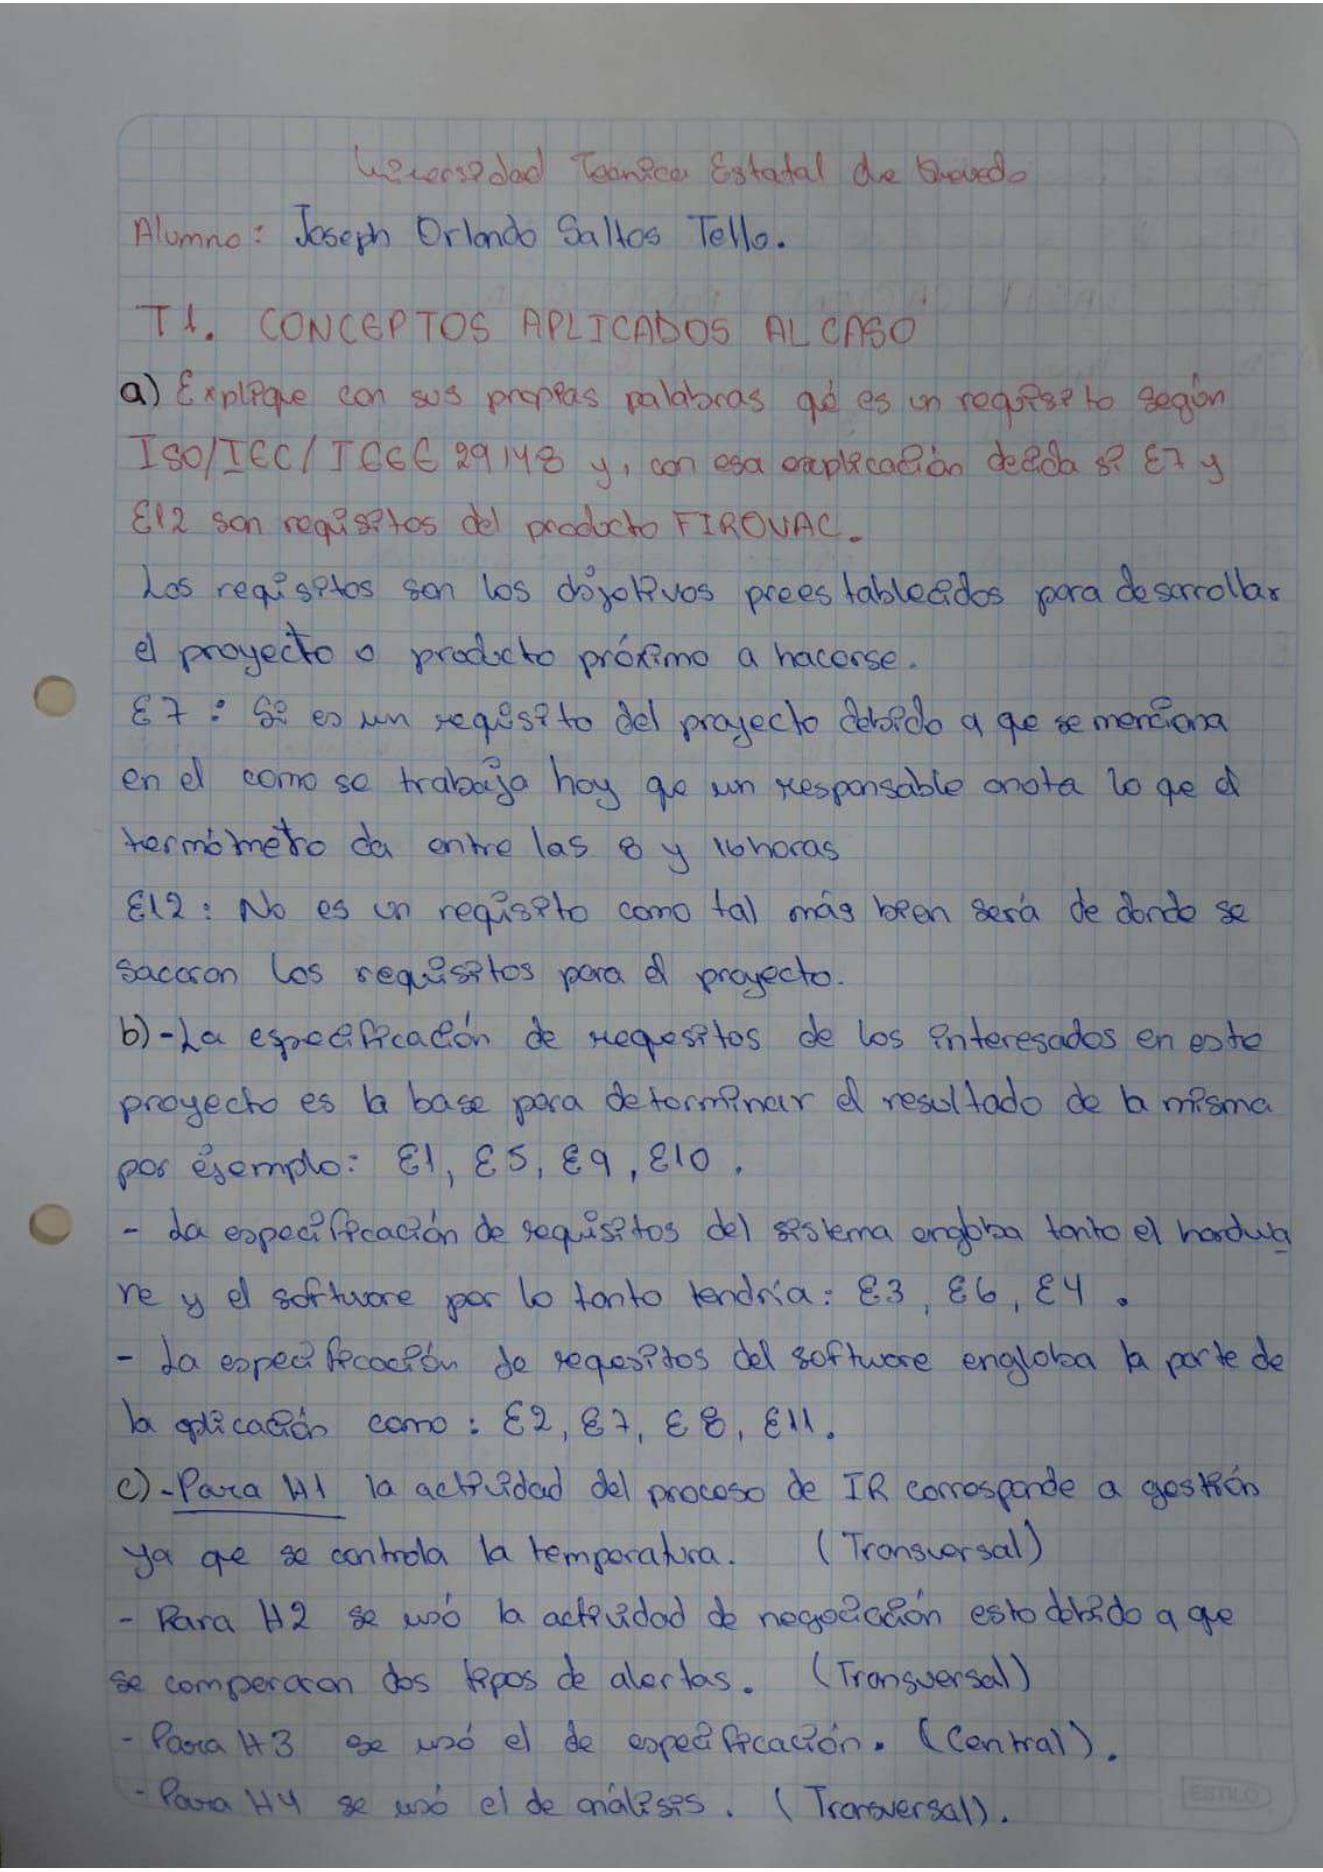
\includegraphics[width=\textwidth,height=0.88\textheight,keepaspectratio]{evidencias/hoja-1.jpg}
		\caption*{Hoja 1}
	\end{figure}
	
	\begin{figure}[H]
		\centering
		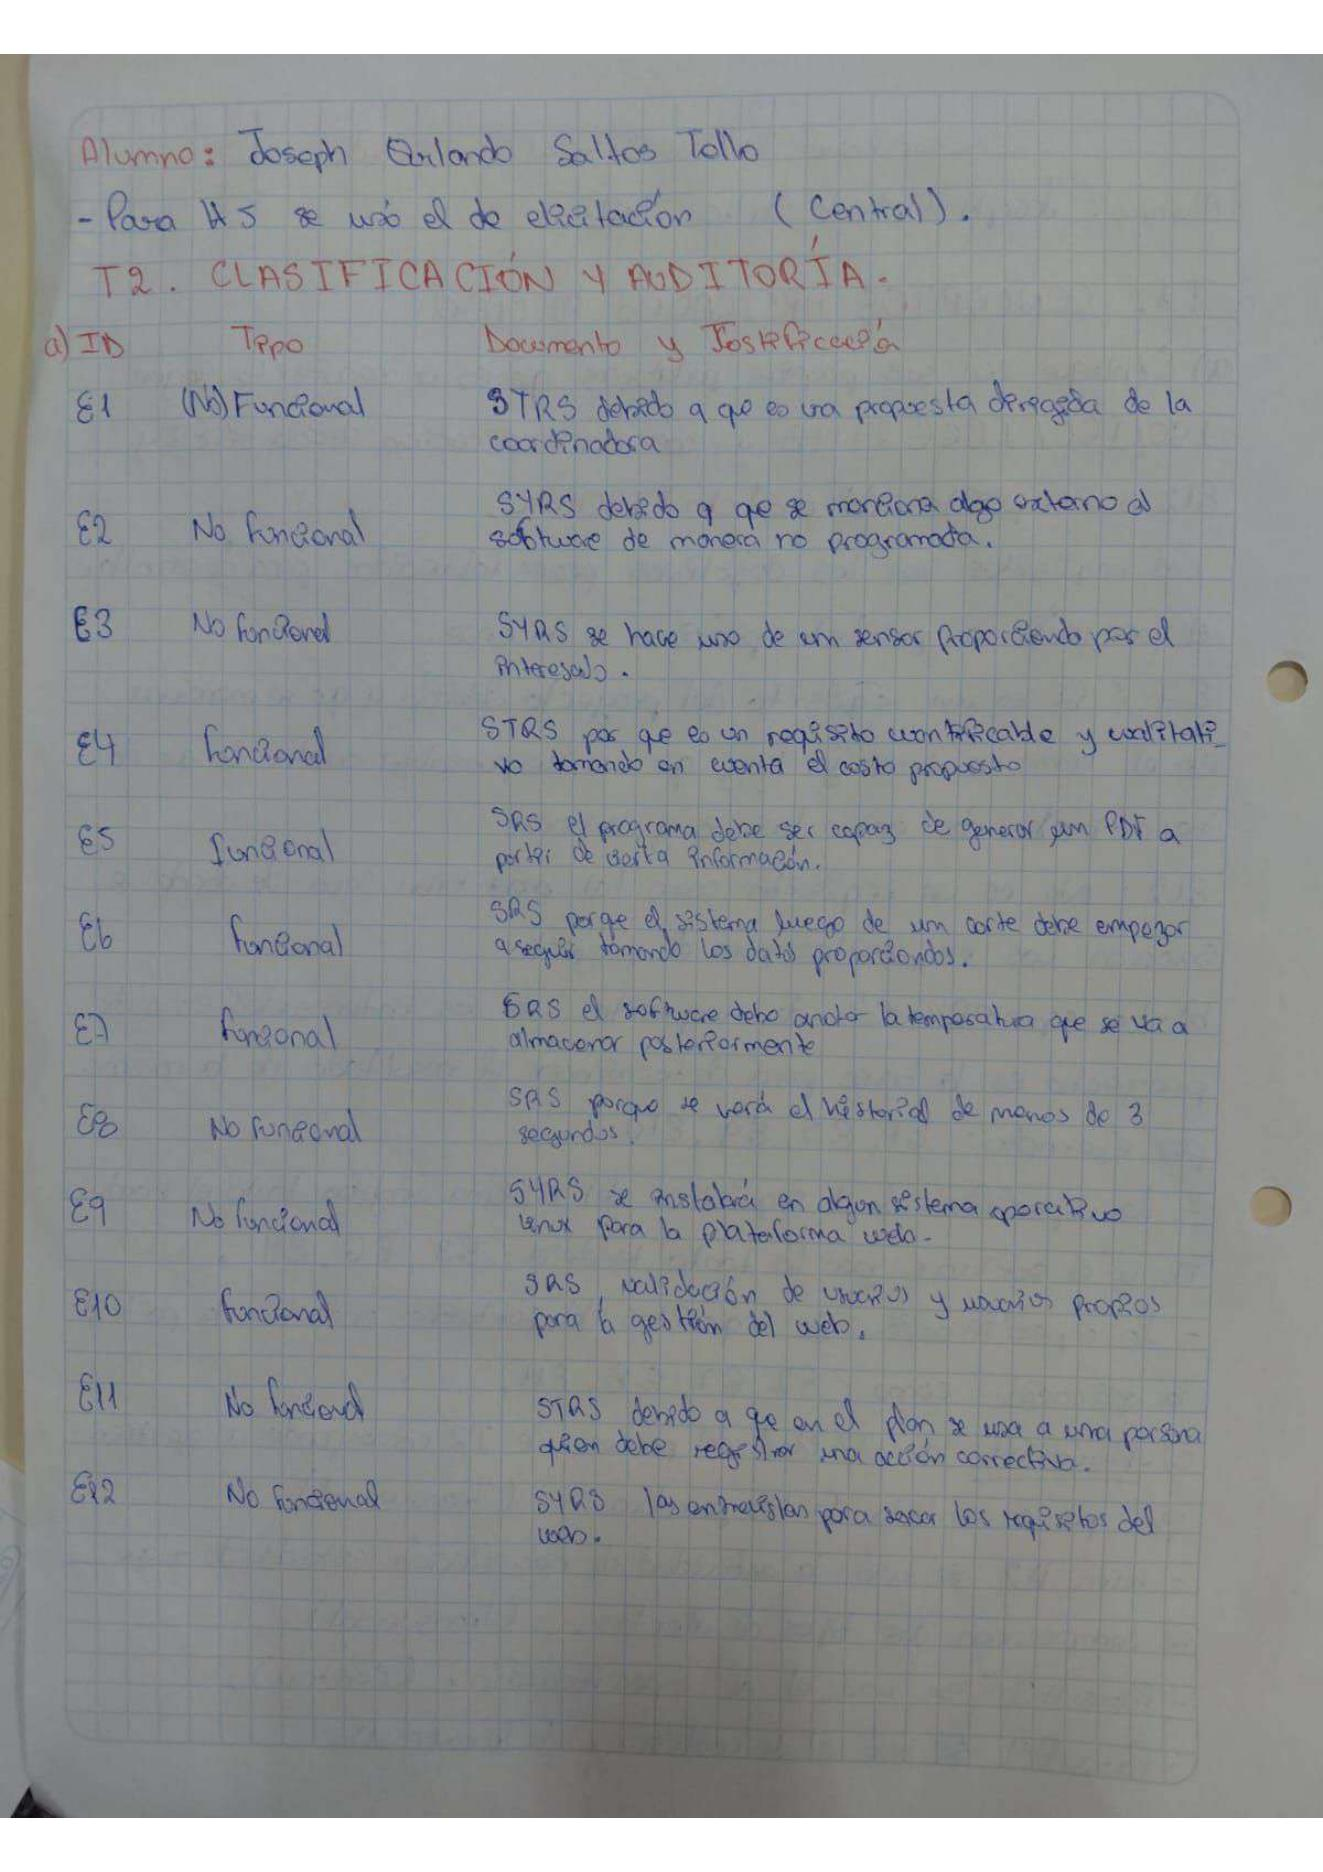
\includegraphics[width=\textwidth,height=0.88\textheight,keepaspectratio]{evidencias/hoja-2.jpg}
		\caption*{Hoja 2}
	\end{figure}
	
	\begin{figure}[H]
		\centering
		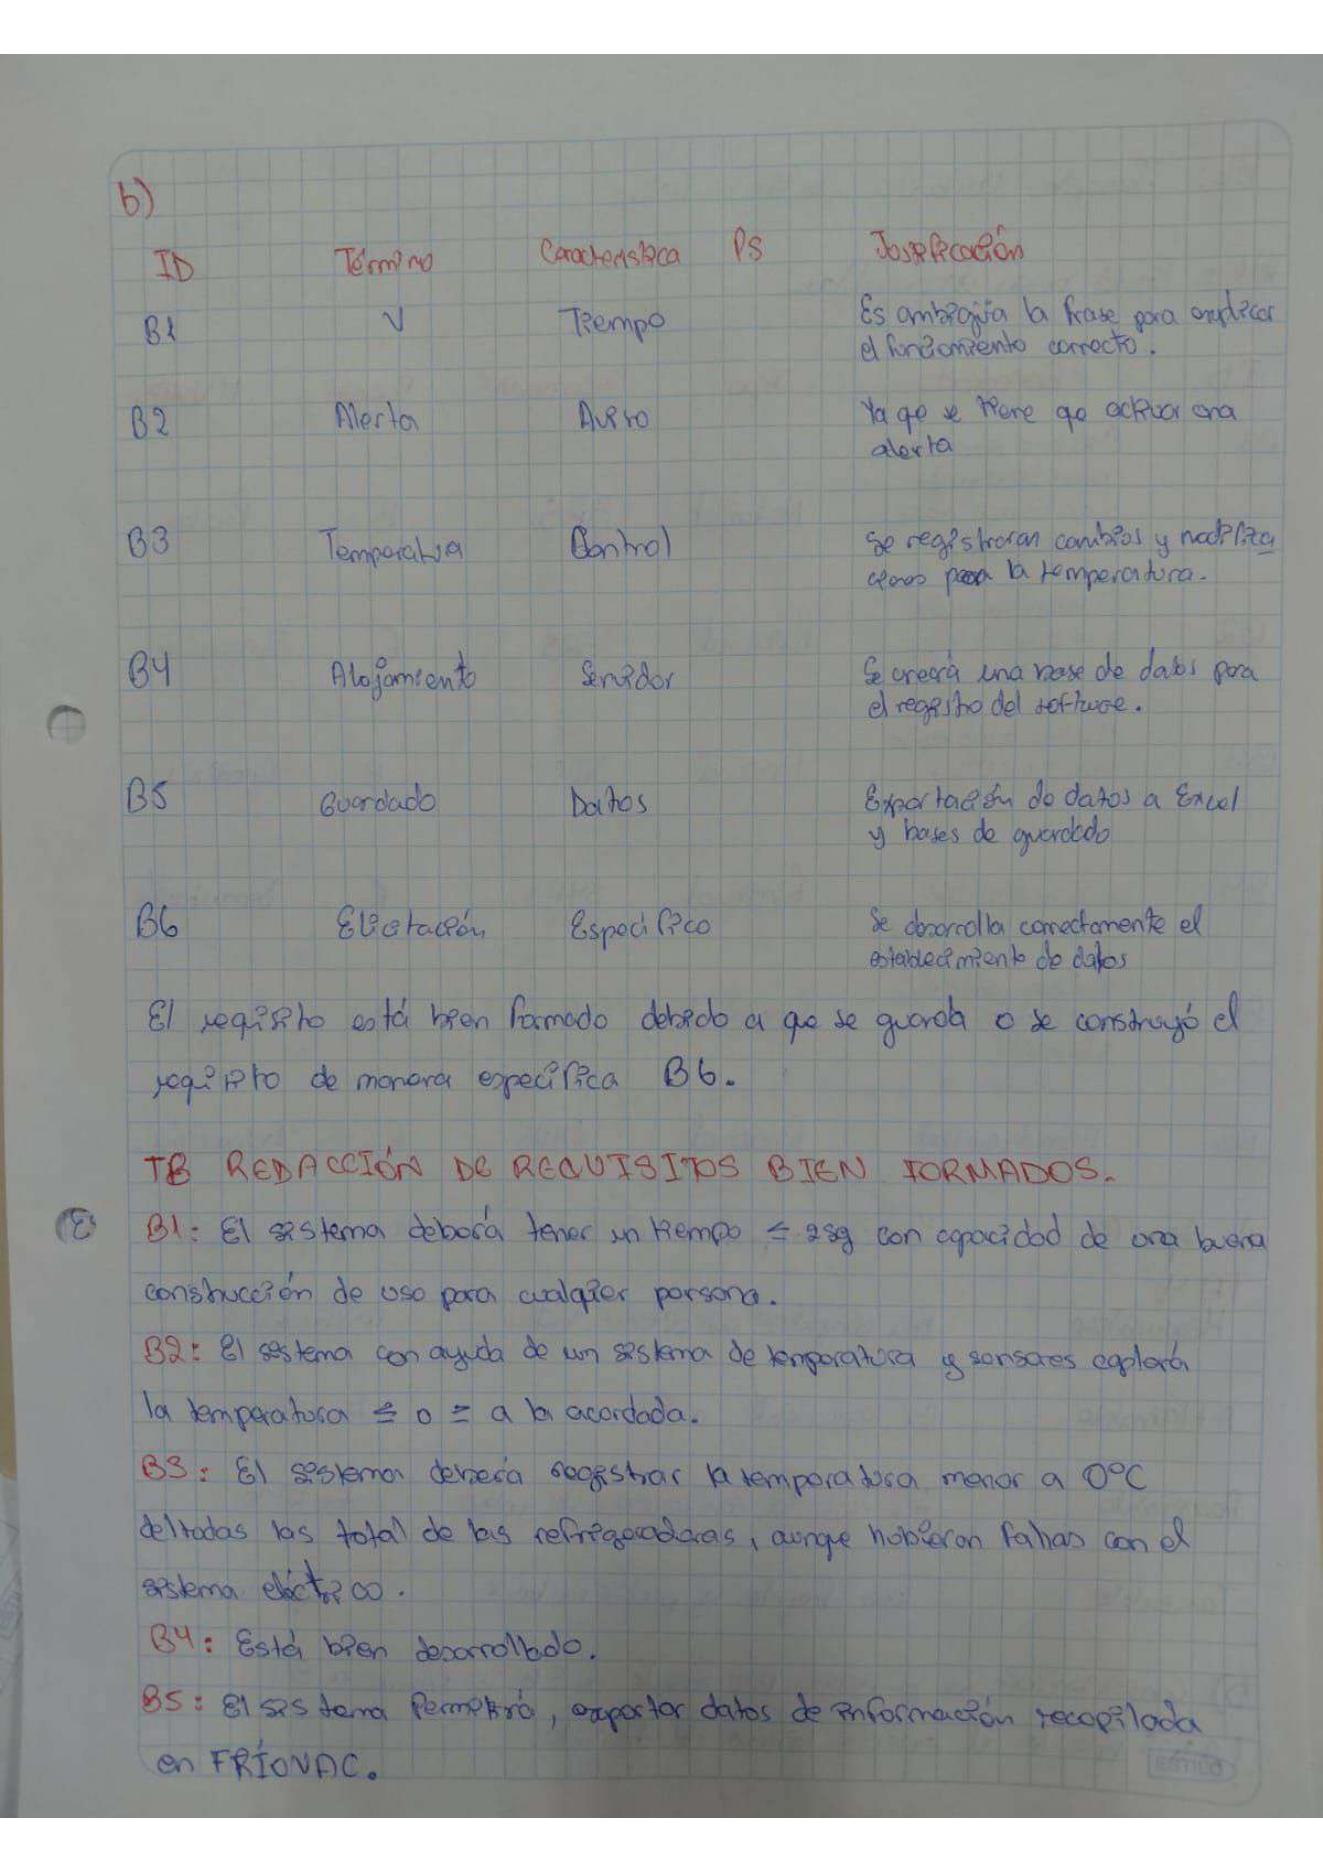
\includegraphics[width=\textwidth,height=0.88\textheight,keepaspectratio]{evidencias/hoja-3.jpg}
		\caption*{Hoja 3}
	\end{figure}
	
	\begin{figure}[H]
		\centering
		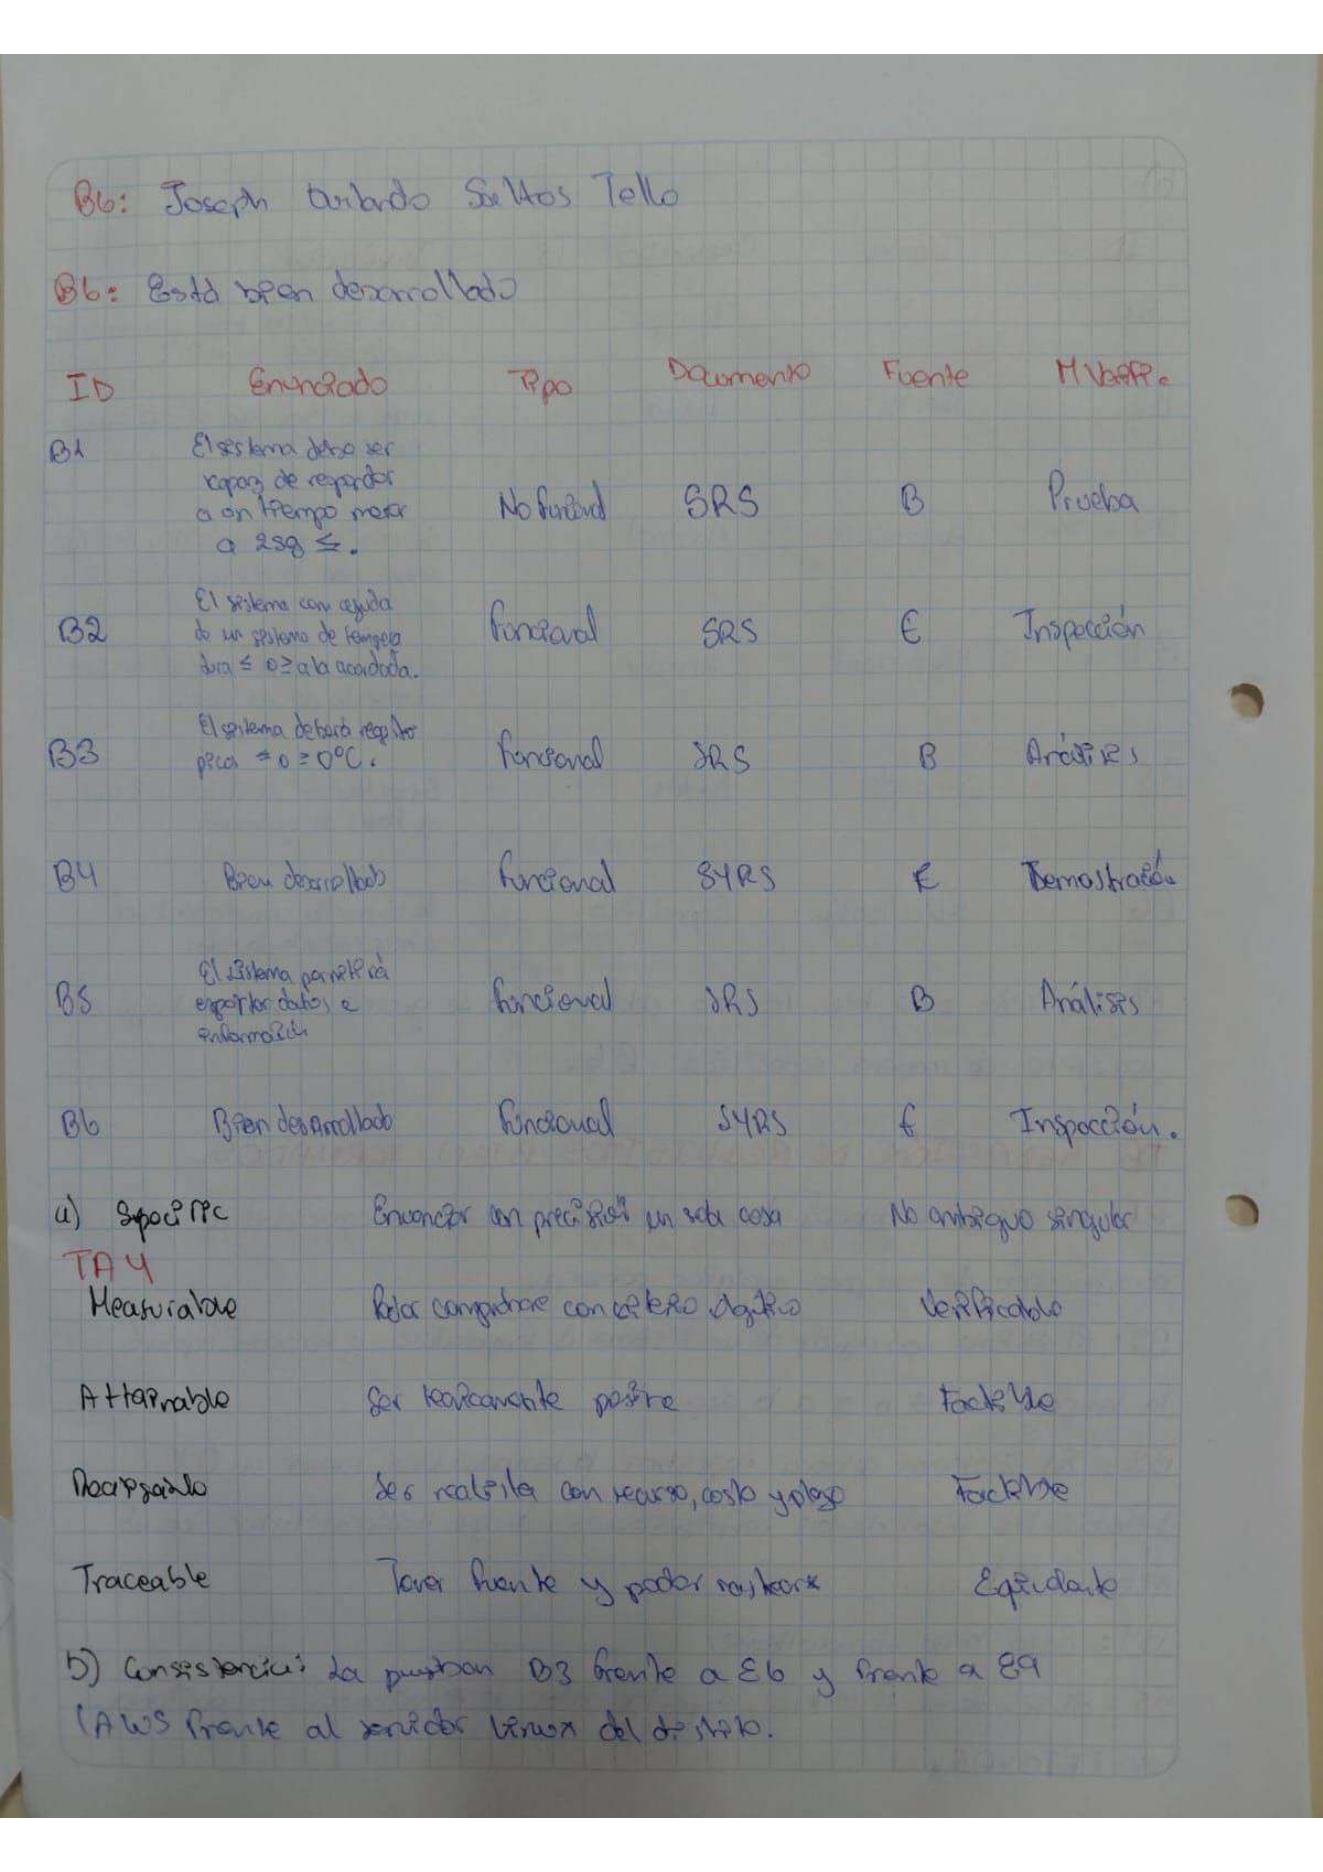
\includegraphics[width=\textwidth,height=0.88\textheight,keepaspectratio]{evidencias/hoja-4.jpg}
		\caption*{Hoja 4}
	\end{figure}
	
\end{document}
